
\section{DWH Implementation}

\begin{breakbox}
\boxtitle{MOLAP:}
\newline Multi-dimensional OLAP stored in n-dimensional arrays.
\begin{center}
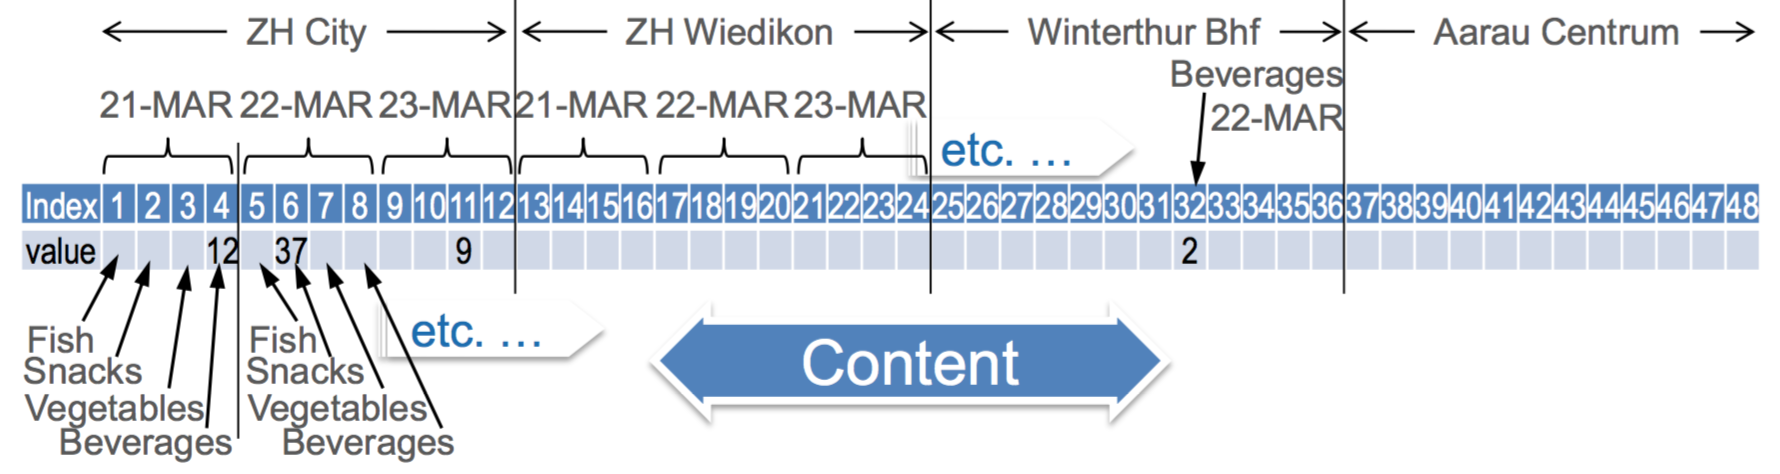
\includegraphics[width=.15\textwidth]{slides_images/molap.png}
\end{center}
Formel für storage (und query):
\begin{center}
$i_{1k} + (i_{2l-1}) \cdot |I_1| + (i_{3m}-1) \cdot |I_1| \cdot |I_2| + \cdots$,
\end{center}
mit $I_j =$ dimension $j$, $i_{jk} =$ index for $k^{th}$ element of dimension $j$.
\end{breakbox}

\begin{breakbox}
\boxtitle{Beispiel (Pages):}
\newline Folgende Tabellen und Daten sind gegeben. Die Dimensionen sind geordnet nach Shipment, Supplier, Year, Product:
\begin{center}
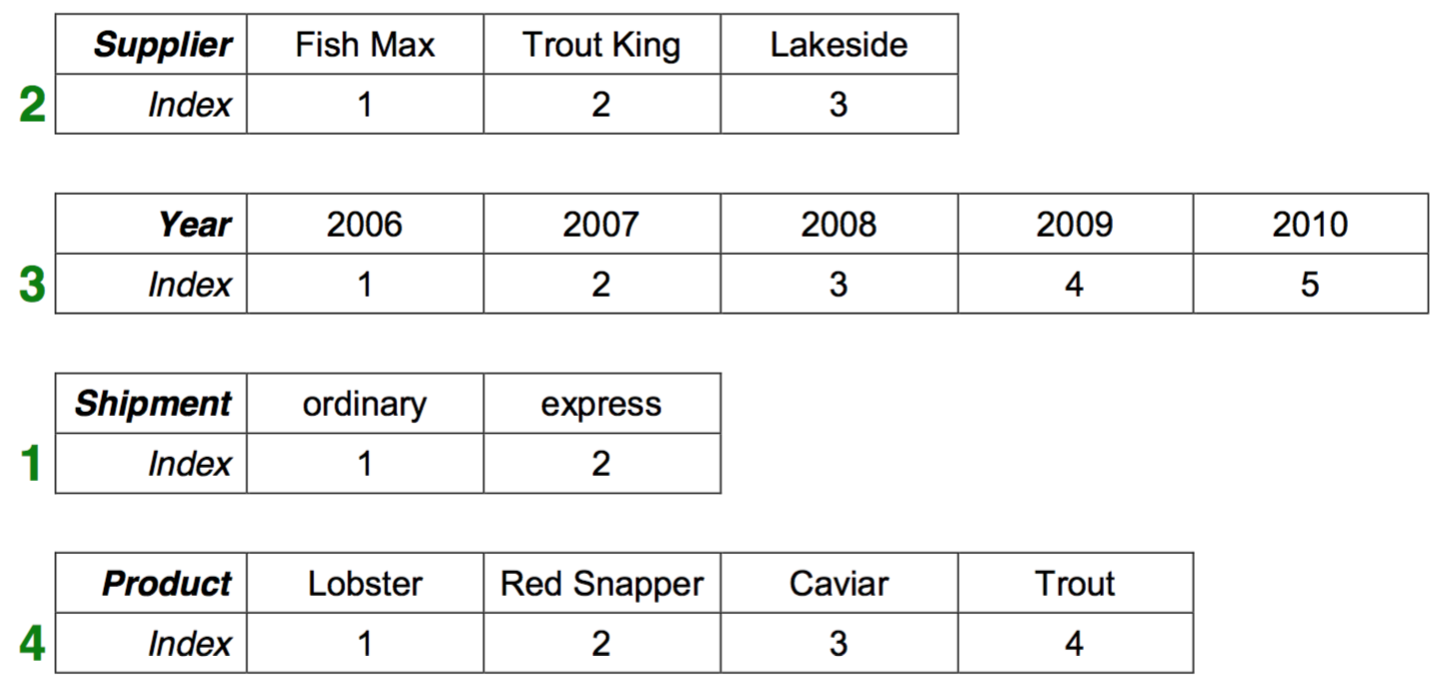
\includegraphics[width=.15\textwidth]{slides_images/molap_example.png}
\end{center}
Aufgabe: A page can hold 4 array cells.
\begin{enumerate}[label=(\alph*)]
	\item How many pages have to be loaded for a query after all sales of Lobster in 2008?
		\begin{itemize}
			\item[] All Lobster array cells adjacent (since it's last dimension in order). Lobster in 2008 spreads over 6 cells (all combinations from Supplier and Shipment dimensions). 6 / 4 = 2 pages.
		\end{itemize}
	\item How many pages have to be loaded for a query after all sales by "express" in 2008?
		\begin{itemize}
			\item[] The 2008 and express combinations spread over 5 cells (i.e. 2 pages), but there are several of those ranges , dispersed over Lobster, Red Snapper, Caviar and Trout. So 4 x 2 = 8 pages.
		\end{itemize}
\end{enumerate}
\begin{center}
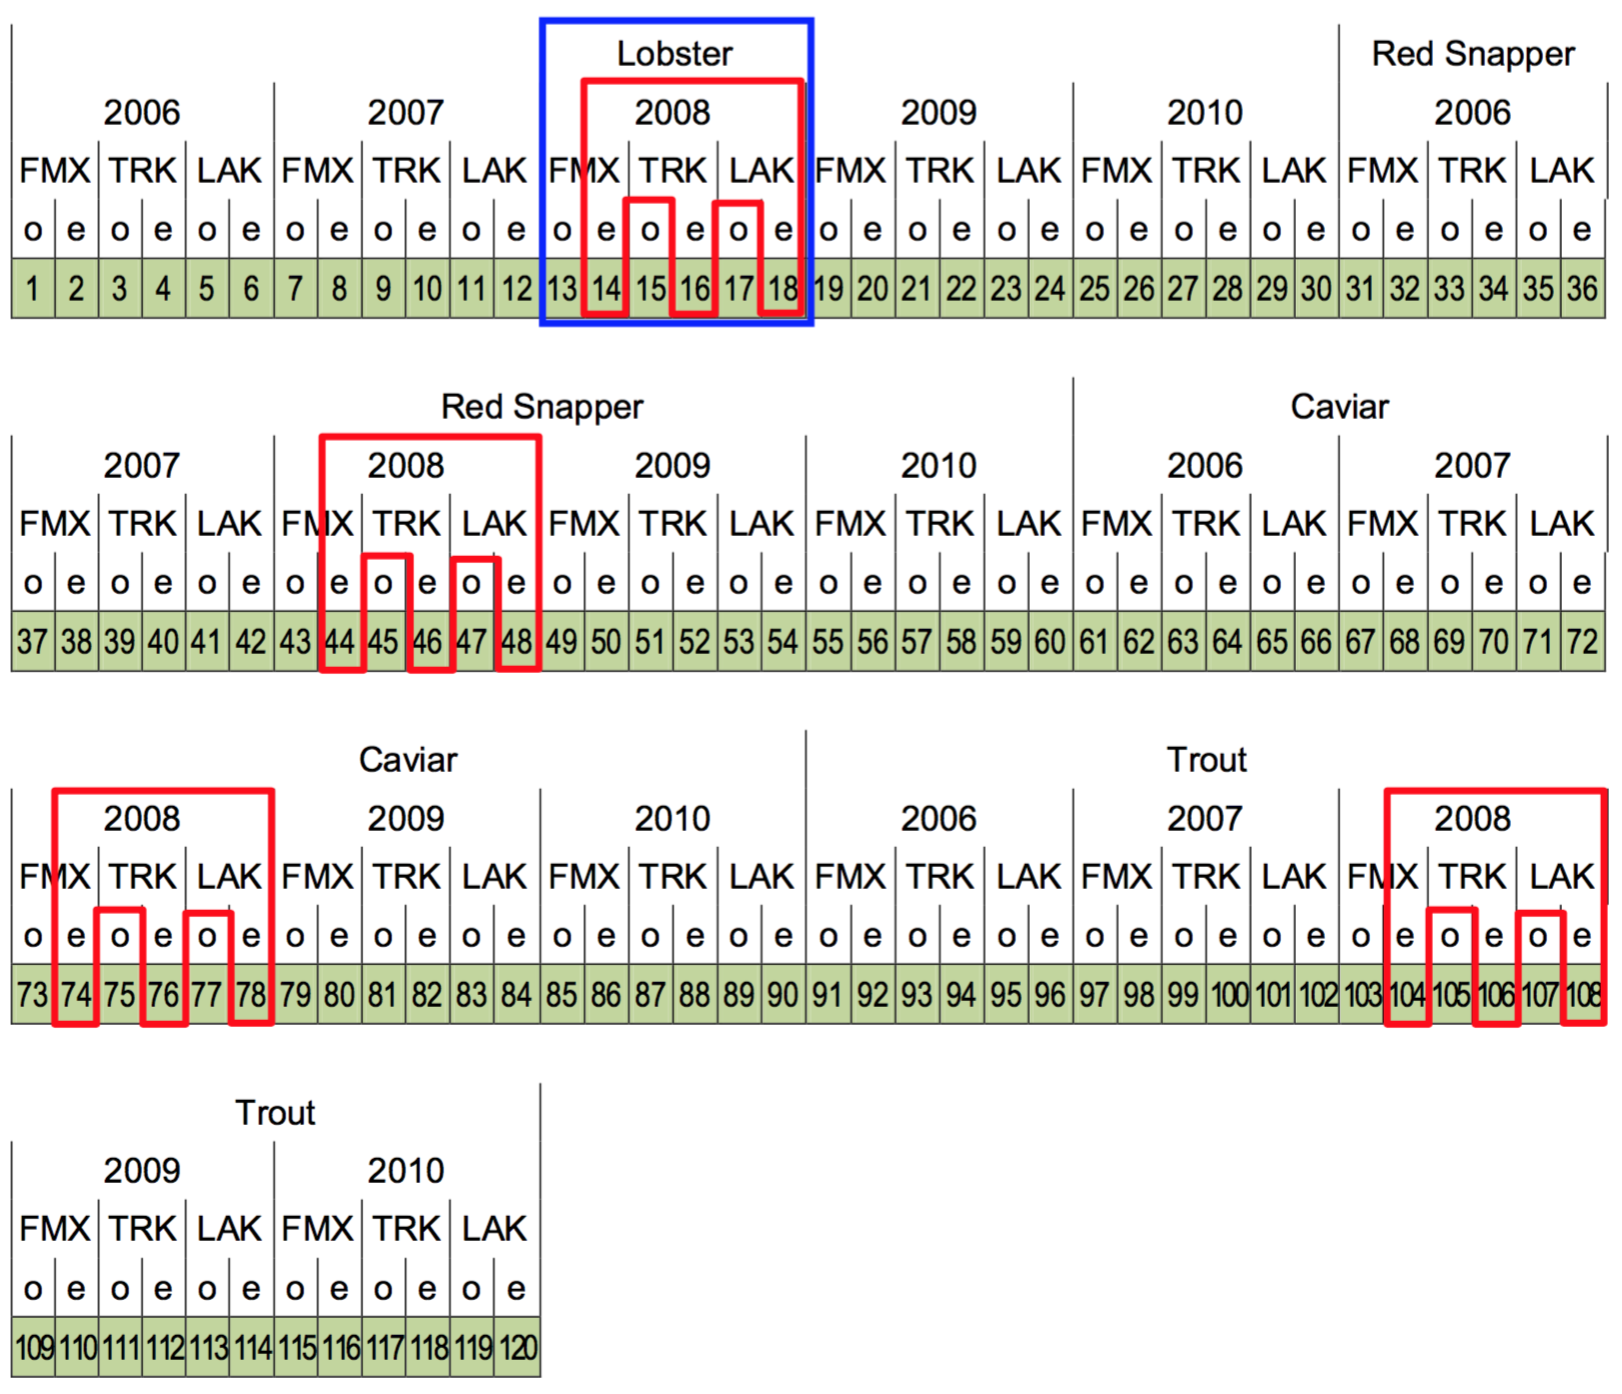
\includegraphics[width=.15\textwidth]{slides_images/molap_solution.png}
\end{center}
\end{breakbox}

\begin{breakbox}
\boxtitle{FASMI:}
\begin{itemize}
	\item \textcolor{Emerald}{F}ast: response time < 5 s, complex queries max. 20 s.
	\item \textcolor{Emerald}{A}nalysis: intuitive analytical functionality.
	\item \textcolor{Emerald}{S}hared: more than 1 user, authorization, authentication.
	\item \textcolor {Emerald}{M}ultidimensional: Multidimensional conceptual view on data.
	\item \textcolor{Emerald}{I}nformation: analysis not limited by OLAP system.
\end{itemize}
\end{breakbox}
\begin{breakbox}
\boxtitle{Optimize MOLAP:}
\newline To address data sparsity MOLAP implementation usually differentiates between:
\begin{itemize}
	\item dense dimensions (e.g. Time, Location, Salesperson).
	\item sparse dimensions (e.g. Customer, Product, Sales Promotion).
	\item dense dimensions form a data block.
	\item sparse dimensions are kept as indexes.
	\item data blocks only exist where sparse dimensions hold values.
\end{itemize}
\begin{center}
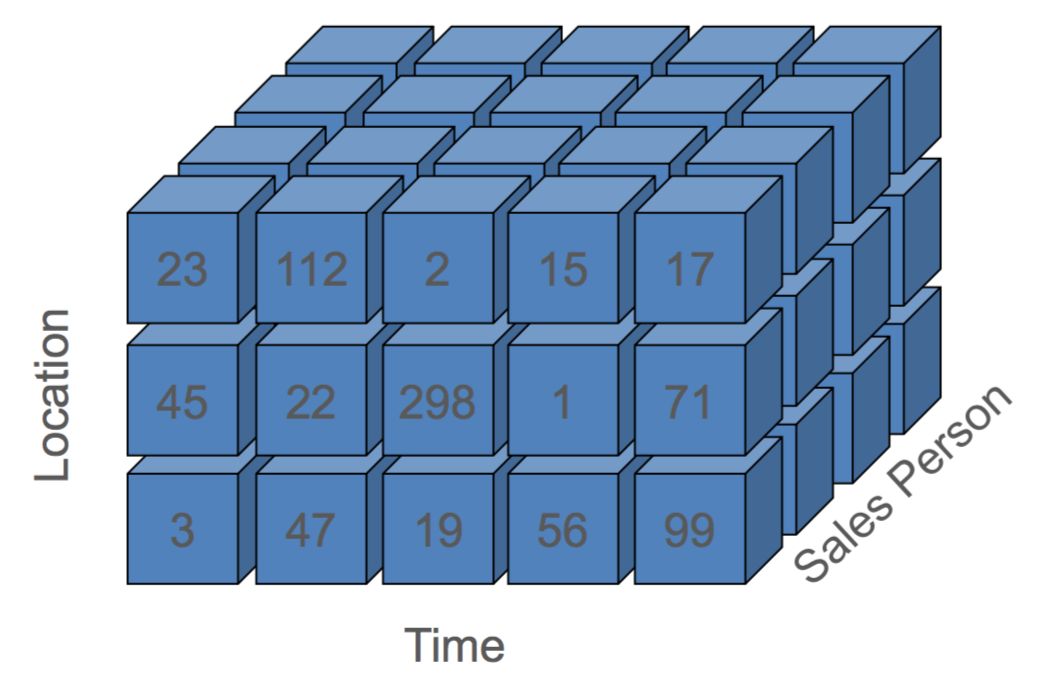
\includegraphics[width=.05\textwidth]{slides_images/dense_molap.png}
\end{center}
\begin{itemize}
	\item data block
	\begin{itemize}
		\item containing individual array cells.
		\item for relatively dense dimensions.
	\end{itemize}
\end{itemize}
\begin{center}
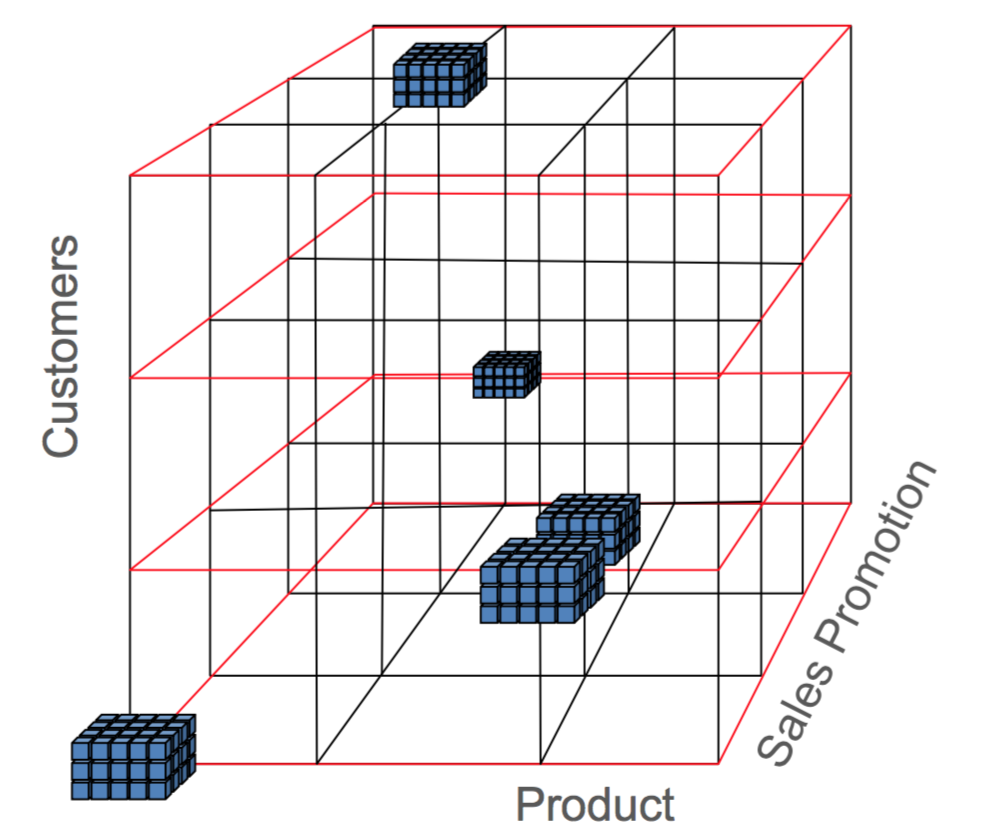
\includegraphics[width=.05\textwidth]{slides_images/sparse_molap.png}
\end{center}
\begin{itemize}
	\item data blocks are only stored for actual occurrences in sparse dimensions.
\end{itemize}
\end{breakbox}

\begin{breakbox}
\boxtitle{MOLAP vs. OLAP:}
\newline MOLAP:
\begin{itemize}
	\item faster computation.
	\item efficiency sensitive to increase in data volume and dimensions.
\end{itemize}
ROLAP:
\begin{itemize}
	\item larger amounts of data.
	\item scalability.
	\item mature DBMSs (concurrency, data management, recovery $\ldots$).
	\item constant transformation necessary between multidimensional $\leftrightarrow$ relational model.
\end{itemize}
\end{breakbox}

\begin{breakbox}
\boxtitle{HOLAP:}
\newline advantage of arrays over relations:
\begin{itemize}
	\item depends on allocation rate of data in cube.
	\item starts at certain thresholds.
\end{itemize}
Objective:
\begin{itemize}
	\item combine advantages of MOLAP and ROLAP.
\end{itemize}
Hybrid OLAP:
\begin{itemize}
	\item hybrid approach.
	\item sparse data remains in relational DB.
	\item dense data gets exported to multidimensional arrays.
\end{itemize}
\end{breakbox}

\begin{breakbox}
\boxtitle{Optimize ROLAP:}
\newline RDBS performance:
\begin{itemize}
	\item suffers most from joins of huge data sets.
\end{itemize}
 Optimization objective:
\begin{itemize}
	\item significantly reduce data sets by indexing.
\end{itemize}
Special indexes often applied with DWHs:
\begin{itemize}
	\item Join Indexes.
	\item Bitmap Indexes.
\end{itemize}
\end{breakbox}

\begin{breakbox}
\boxtitle{Join Indexes:}
\begin{center}
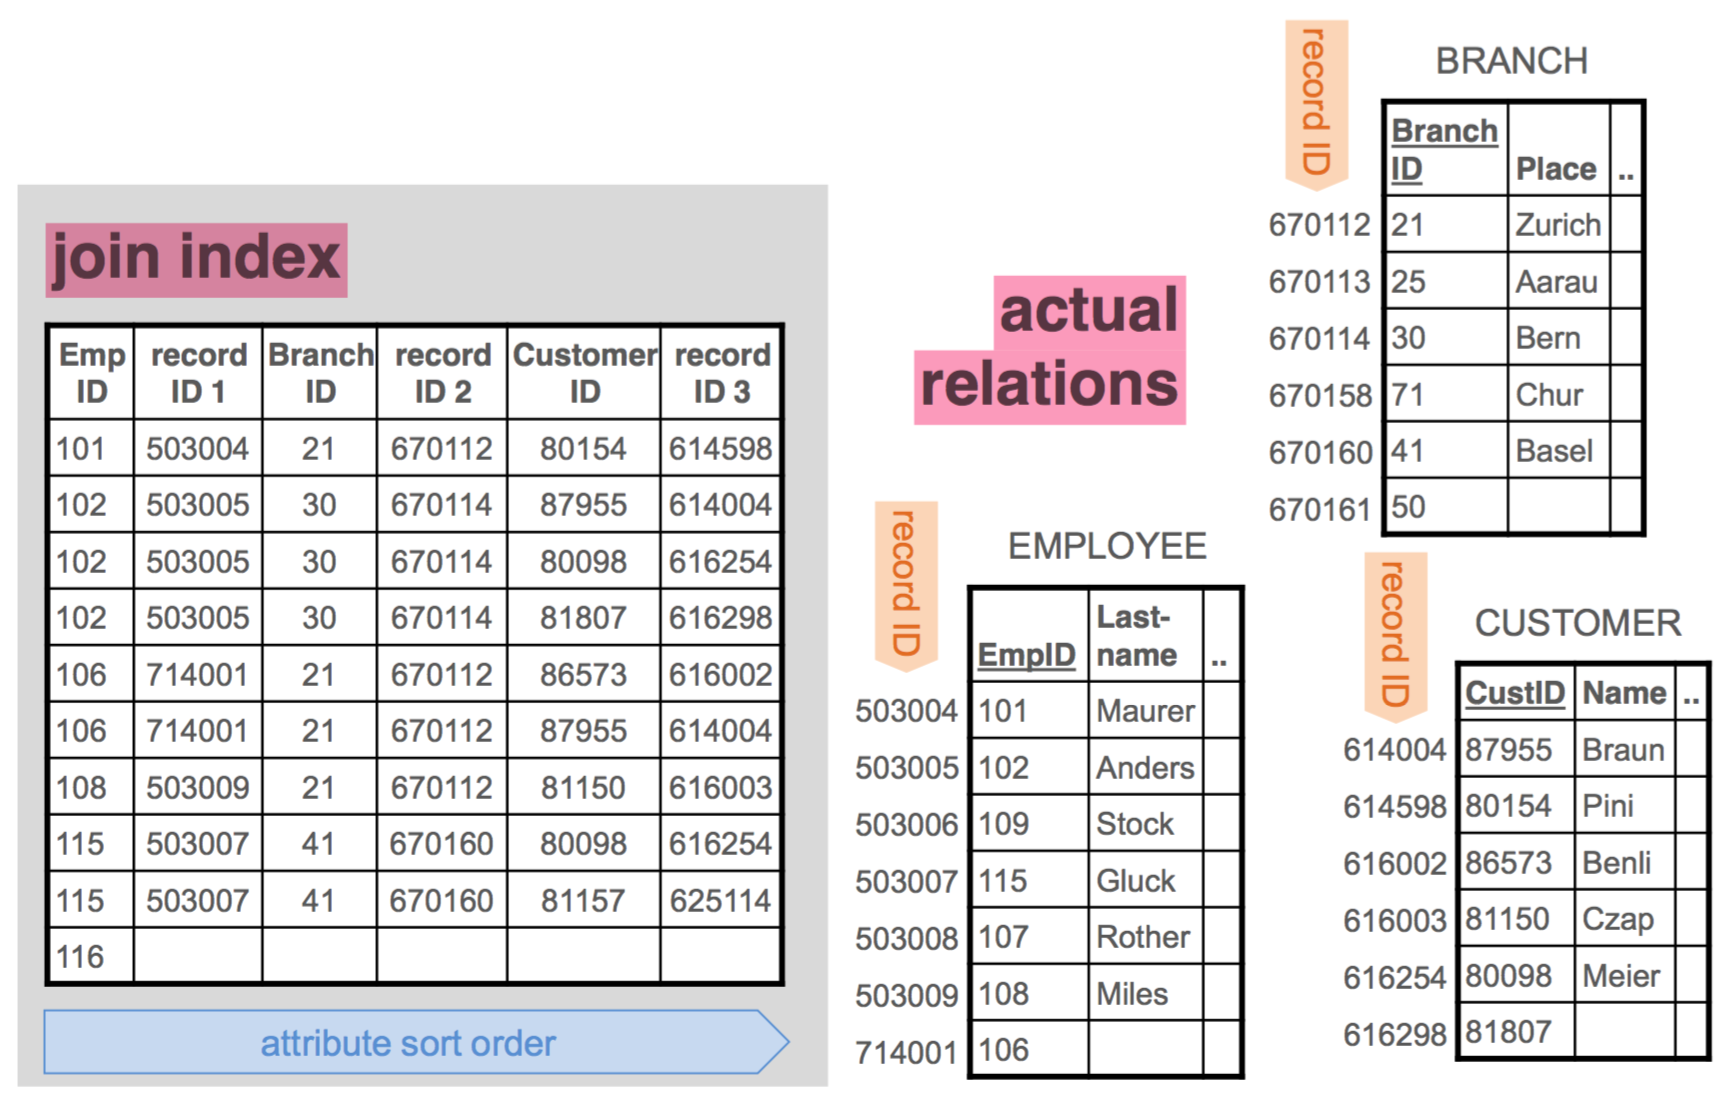
\includegraphics[width=.15\textwidth]{slides_images/join_indexes.png}
\end{center}
\begin{itemize}
	\item combine record IDs for attributes in multiple tables at a time.
	\item create indexes for every such attribute combination frequently used for joins
	\begin{itemize}
		\item e.g. dimension attributes
		\item combinational explosion!
	\end{itemize}
	\item sort order of attributes impacts query acceleration.
\end{itemize}
\end{breakbox}

















